\section{Theorie}
\label{sec:Theorie}

In der Quantenelektrodynamik sind das Korpuskel- als auch das Wellenmodell als Grenzfälle enthalten.
Um den Photoeffekt, also das Auslösen von Elektronen durch Bestrahlung mit Licht, zu beschreiben 
muss jedoch das Korpuskelmodell gewählt werden, da das Wellenmodell zu Vorhersagen führt, die so nicht 
beobachtet werden können. Dazu gehört, dass theoretisch die Elektronen emittiert werden müssten, sobald sie 
die elektrostatischen, rücktreibenden Kräfte überwinden können. Die Energie der Elektronen müsste außerdem 
mit zunehmender Intensität anwachsen. Experimentell lassen sich jedoch die folgenden Aussagen bestätigen, 
welche durch das Korpuskelmodell zu erläutern sind: 
 \begin{enumerate}
    \item Die Anzahl der Elektronen ist proportional zur Intensität.
    \item Die Elektronenenergie ist proportional zur Frequenz und unabhängig von der Intensität.
    \item Es existiert eine Grenzfrequenz, unterhalb der der Photoeffekt nicht auftritt. 
 \end{enumerate}

 Bei der Korpuskeltheorie wird angenommen, dass die Energie von Licht in Photonen quantisiert ist.
 Nach Einstein verhalten sich Lichtquanten wie Plancksche Energiequanten. Das heißt, dass sich 
 monochromatisches Licht mit der Frequenz $\nu$ geradlinig mit der Lichtgeschwindigkeit c bewegt. 
 Alle Photonen haben dann die Energie $\symup{h}\nu$. Desweiteren teilt sich die Photonenenergie bei 
 Übertrag auf ein Elektron auf die Austrittsarbeit $A_{\symup{k}}$ und die kinetische Energie des 
 Elektrons auf
\begin{equation}
    \symup{h} \nu = E_{\symup{kin}} + A_{\symup{k}} \; .
    \label{eqn:energie}
\end{equation}
Daraus folgt, dass der Photoeffekt nicht mehr auftreten kann, wenn die Energie des Photons 
kleiner als die Austrittsarbeit ist. Die emittierten Elektronen folgen der Fermi-Dirac-Verteilung, d.h. 
dass deren Austrittsgeschwindigkeiten aufgrund vorheriger Energien statistisch verteilt sind.
 Außerdem lässt sich aus \autoref{eqn:energie} erkennen, 
dass die kinetische Energie proportional zur Frequenz ist. Die Lichtintensität ist in allgemeinen 
proportional zur Photonenanzahl. Da jedes Photon maximal ein Elektron auslösen kann, ist die Intensität 
auch proportional zur Anzahl der ausgelösten Elektronen.

\subsection{Untersuchung mit der Gegenfeldmethode}
Um die kinetische Energie der Elektronen zu messen, muss die Photozelle wie in \autoref{fig:gegenfeld} 
um ein Voltmeter und ein Picoamperemeter erweitert werden.
\begin{figure}
    \centering
    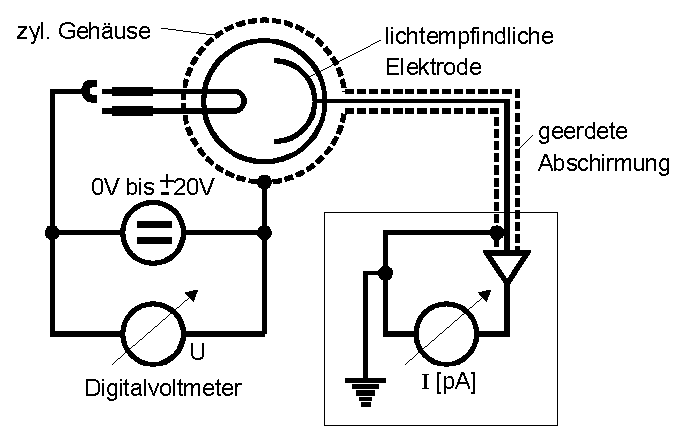
\includegraphics[height = 6cm]{gegenfeld.pdf}
    \caption{Aufbau der Messapparatur zur Messung mit der Gegenfeldmethode \cite{ap500}.}
    \label{fig:gegenfeld}
\end{figure}
Durch das angelegte Gegenfeld an der Anode
können nur die Elektronen die Anode erreichen, dessen kinetische Energie größer als $\symup{e_0}U_{\symup{g}}$
ist. Bei 
\begin{equation*}
    \symup{e_0}U_{\symup{g}} = \frac{1}{2} m_0 v_{\symup{max}}^2
\end{equation*}
verschwindet somit der Strom. Es lässt sich also die kinetische Energie der schnellsten Elektronen 
berechnen
\begin{equation}
    \symup{h} \nu = \symup{e_0}U_{\symup{g}}  + A_{\symup{k}} \; .
    \label{eqn:nu}
\end{equation}
In der Praxis verschwindet der Photostrom nicht schlagartig bei $U_{\symup{g}}$, sondern sinkt bereits 
bei kleineren Spannungen ab. Der typische Verlauf der Strom-Spannungskurve ist in \autoref{fig:energie}
dargestellt. 
\begin{figure}
    \centering
    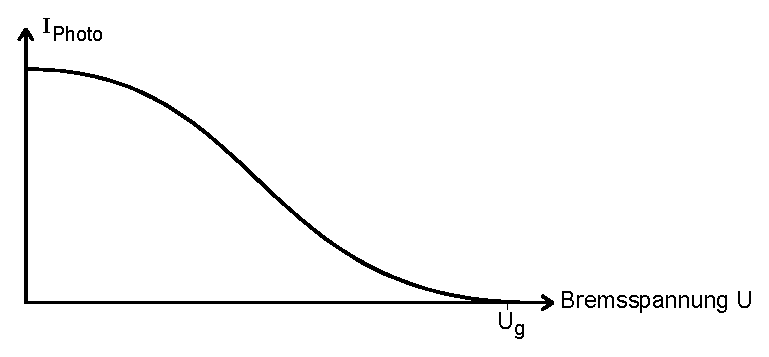
\includegraphics[height = 6cm]{energie.pdf}
    \caption{Photostrom in Abhängigkeit von der Bremsspannung \cite{ap500}.}
    \label{fig:energie}
\end{figure}
Zwischen dem Photostrom und der Spannung gilt ein parabolischer Zusammenhang
\begin{equation*}
    I_{\symup{Ph}} \propto U^2 \; .
\end{equation*}
Desweiteren tritt nur ein Photostrom auf, wenn die Elektronen eine höhere Energie haben als die Austrittsarbeit 
der Anode ist. In manchen Fällen lässt sich also erst ein Photostrom detektieren, wenn eine beschleunigende 
Spannung angelegt wird. Ein negativer Strom wird dann gemessen, wenn die Bremsspannung hinreichend hoch 
ist und sich dieser Strom mit dem Photostrom von der Kathode kommend überlagert.